\section{Tipos de sensores}
\textbf{Por posición:}

\textbf{Encoder Incremental:} Este tipo de sensor óptico digital convierte el movimiento en una secuencia de pulsos digitales. Tiene una escala transparente con una retícula opaca; de un lado, tiene una escala equipada con una fuente de luz y un lente condensador. Del otro lado, hay celdas sensibles a la luz. La manera en la que funciona es que la resistencia de las celdas disminuye cada vez que reciben un rayo de luz, de este modo se genera un pulso cada vez que un rayo de luz es atravesado.\autoref{fig:20150317193931229}

considerable.\autoref{fig:lvdt} \\
\begin{figure}[h]
	\centering
	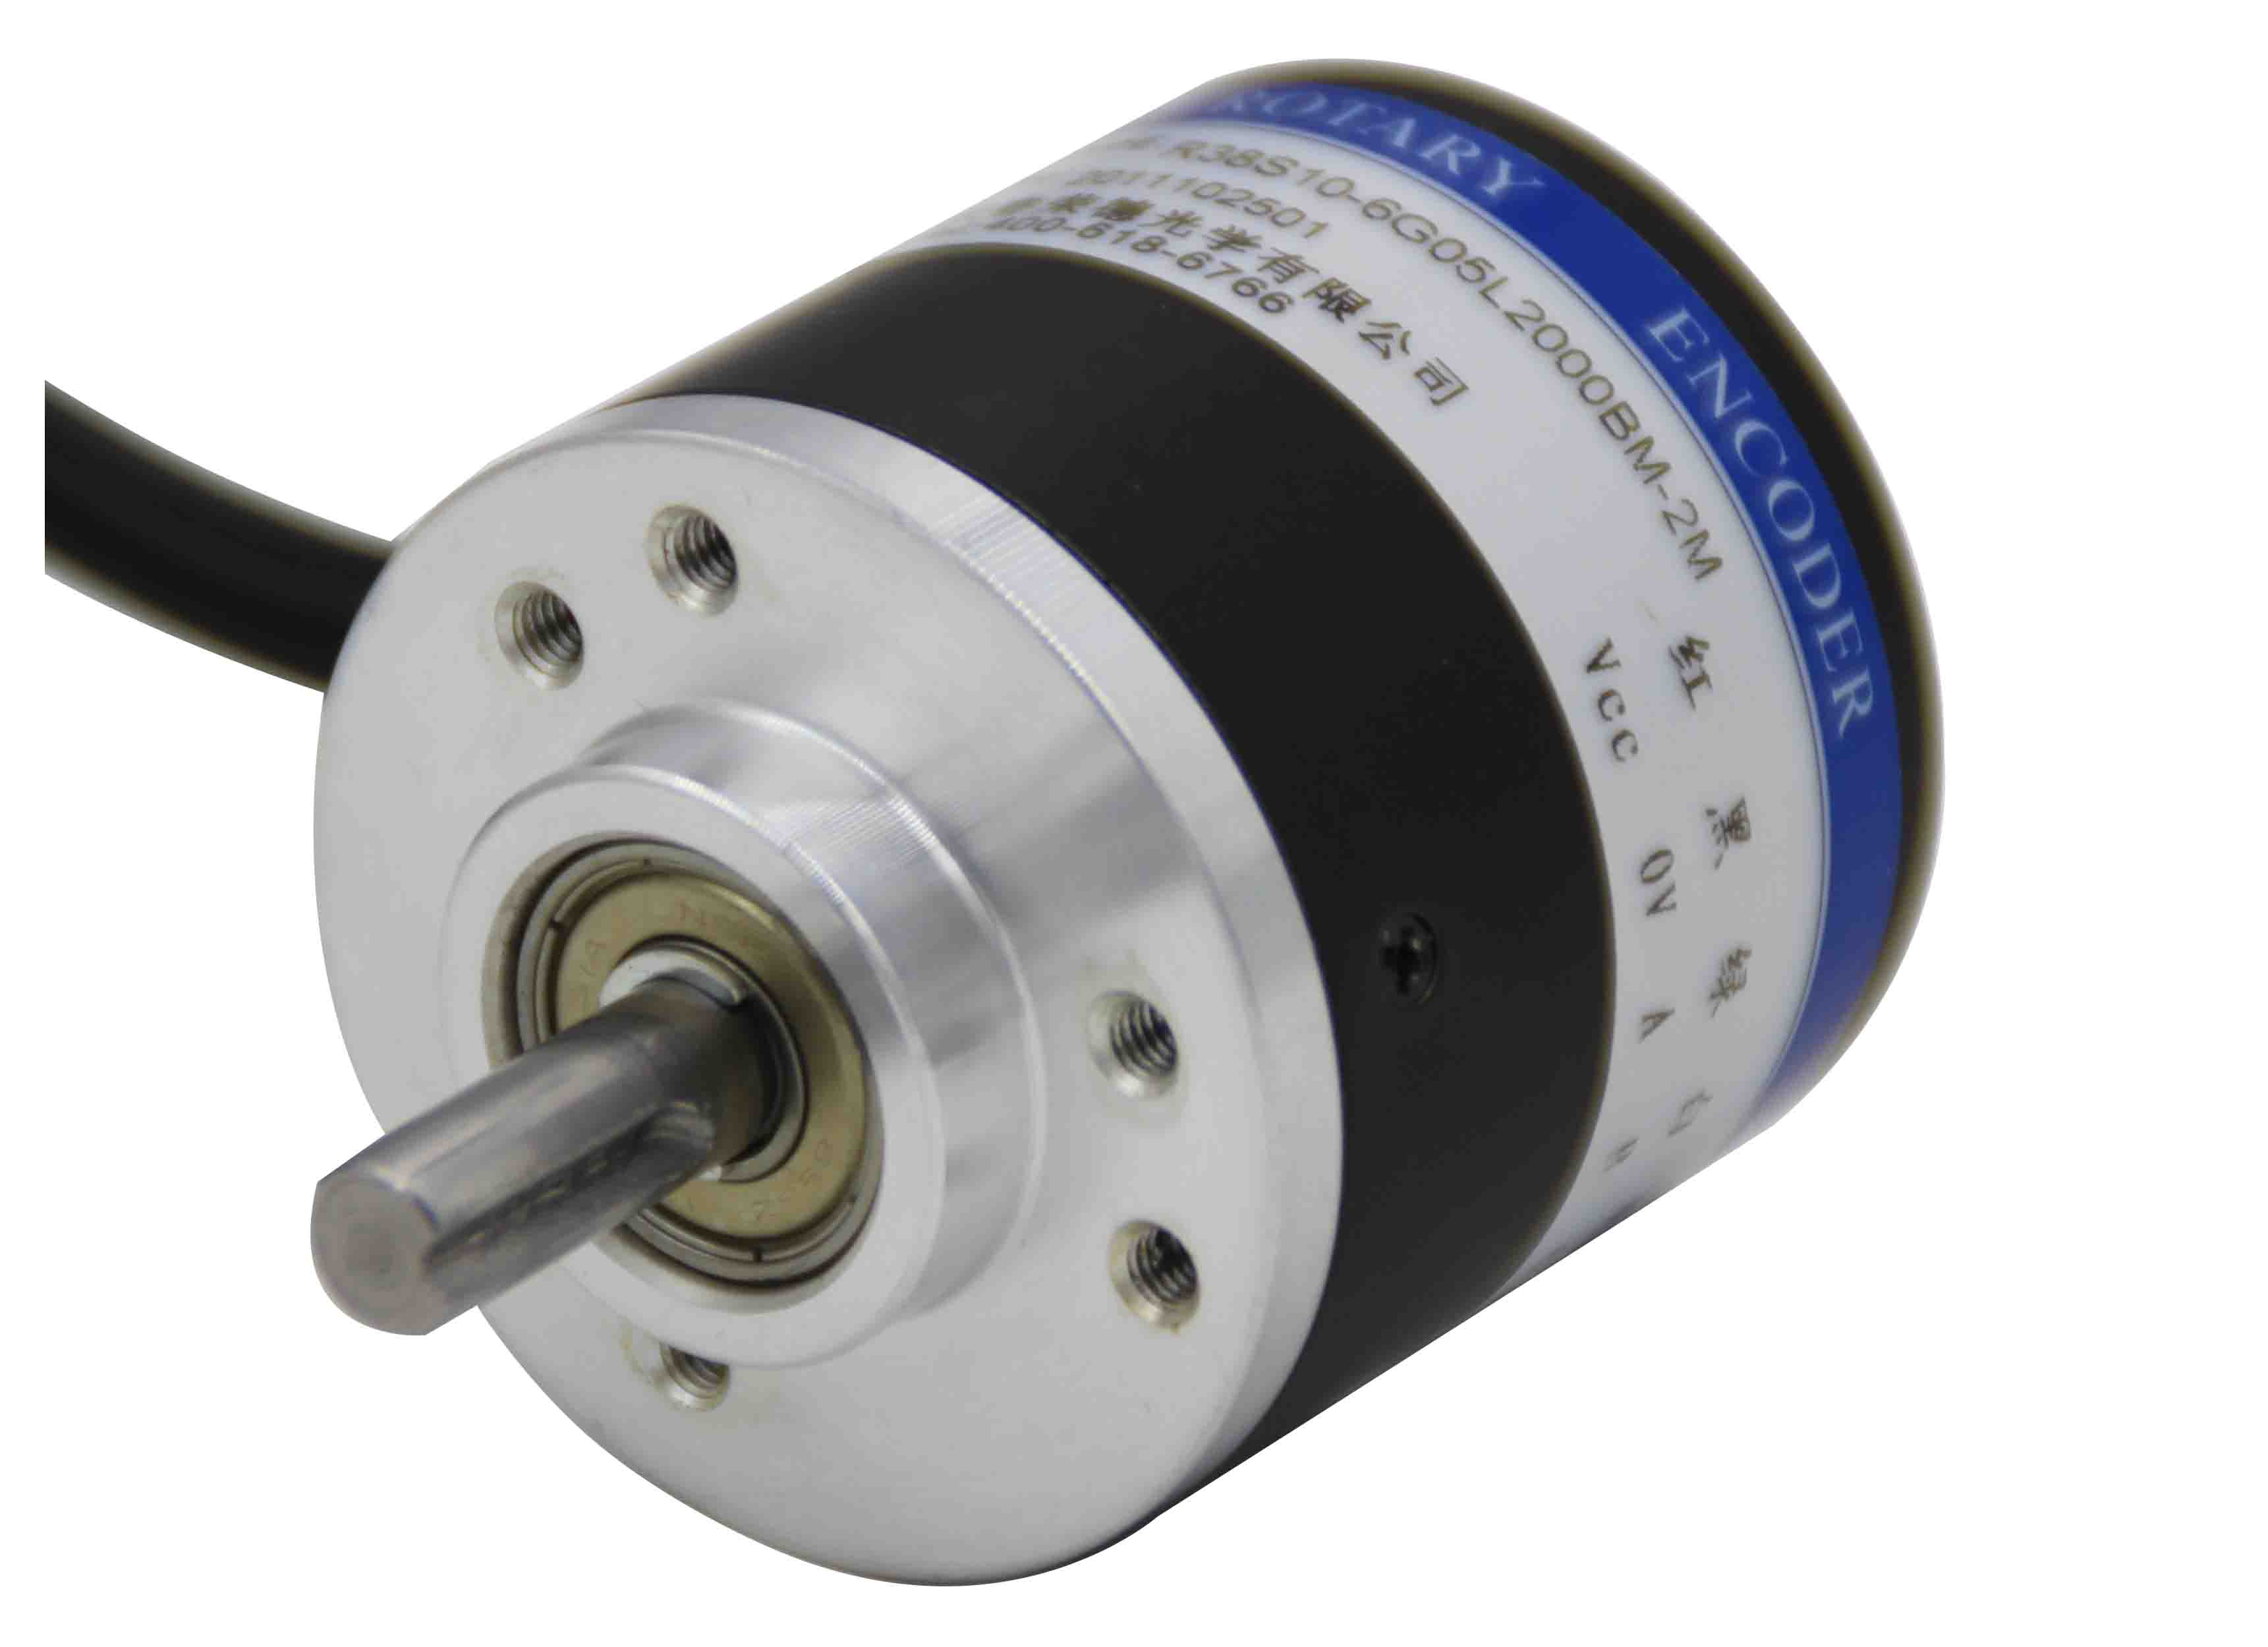
\includegraphics[width=0.4\linewidth]{portada/20150317193931229}
	\caption{}
	\label{fig:20150317193931229}
\end{figure}

\textbf{Potenciómetro:} Es un dispositivo de resistencia variable que expresa desplazamientos lineales o angulares en términos de voltaje. Consiste en una clavija deslizante que hace contacto con un elemento resistivo, conforme se mueve este punto de contacto la resistencia entre el contacto deslizante y las conexiones de los extremos del dispositivos cambia en proporción al desplazamiento. \autoref{fig:potenciometro}\\\\\\\\\\\\\\\\\\

\begin{figure}[h]
	\centering
	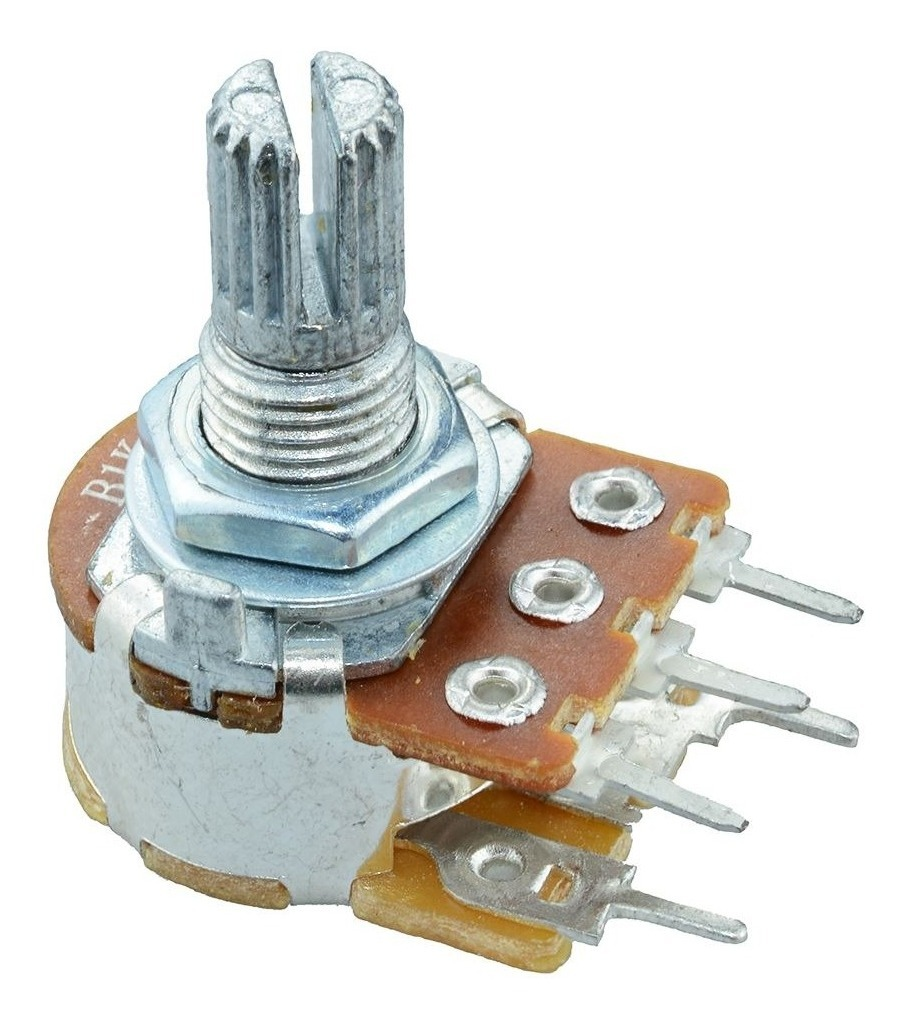
\includegraphics[width=0.2\linewidth, height=0.2\textheight]{img/potenciometro}
	\caption[Potenciómetro]{}
	\label{fig:potenciometro}
\end{figure}



\textbf{LVDT:} Es uno de los transductores de desplazamiento más populares ya que genera una señal de CA cuya magnitud se relaciona con el desplazamiento de un núcleo móvil. Tiene como concepto básico de un núcleo móvil rodeado por dos bobinas secundarias y una bobina principal y conforme el núcleo cambia su posición con respecto a las bobinas cambia también el campo magnético y por tanto se modifica la amplitud de voltaje en la bobina secundaria como una función del desplazamiento del núcleo a través de un segmento 



\begin{figure}[h]
	\centering
	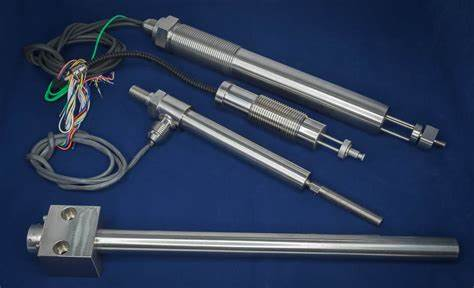
\includegraphics[width=0.2\linewidth, height=0.2\textheight]{img/LVDT}
	\caption{}
	\label{fig:lvdt}
\end{figure}




\textbf{Resolver:} Son sensores que proporcionan señales análogas como salidas y consisten en un eje (flecha) giratoria (rotor) y una carcasa estacionaria. Sus señales tienen que convertirse a la forma digital por medio de un convertidor analógico a digital. Los resólvers tienen dos devanados orientados a 90°. \autoref{fig:resolver}

\begin{figure}[!]
	\centering
	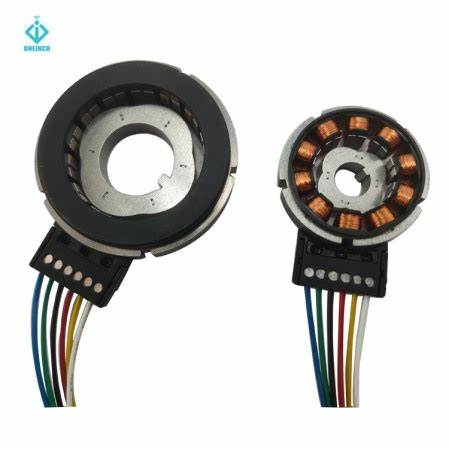
\includegraphics[width=0.2\linewidth, height=0.15\textheight]{img/resolver}
	\caption[Resolver]{}
	\label{fig:resolver}
\end{figure}


\begin{document}
	
	\textbf{Velocidad-tacogeneratriz :}
	
	La captación de la velocidad se hace necesaria para mejorar el comportamiento dinámico de los actuadores del robot. La velocidad de movimiento de cada actuador (que tras el reductor es la velocidad de la articulación) se realimenta normalmente a un bucle de control analógico implementado en el propio accionador del elemento motor. No obstante, en ocasiones en las que el sistema de control del robot lo exija, la velocidad de giro de cada actuador es llevada hasta la unidad de control del robot. Normalmente, y puesto que el bucle de control de velocidad es analógico, el captador usado es una tacogeneratriz que proporciona una tensión proporcional a la velocidad de giro de su eje (valores típicos pueden ser 10 milivoltios por rpm). Otra posibilidad, usada para el caso de que la unidad de control del robot precise valorar la velocidad de giro de las articulaciones, consiste en derivar la información de posición que ésta posee.\autoref{fig:oip}
	
	

	\begin{figure}[h]
	\centering
	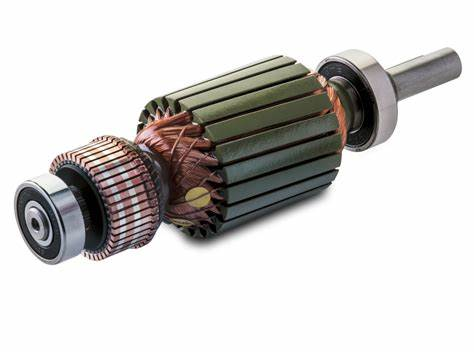
\includegraphics[width=0.2\linewidth, height=0.2\textheight]{img/OIP}
	\caption{}
	\label{fig:oip}
	\end{figure}
	
	\textbf{Tacometro:}
	
	Estos sensores pueden encontrar directamente la velocidad en cualquier momento ya que estos miden la velocidad de rotación de un elemento. Su diseño se basa en la regla de Fleming que declara que “el voltaje producido es proporcional al índice del acoplamiento inductivo”. Aquí un conductor (básicamente una bobina) se sujeta al elemento rotativo que gira en un campo magnético (estator). Conforme incrementa la velocidad del eje, el voltaje producido en las terminales de las bobinas también aumenta.\autoref{fig:tacometro}
	
	
\begin{figure}[h]
	\centering
	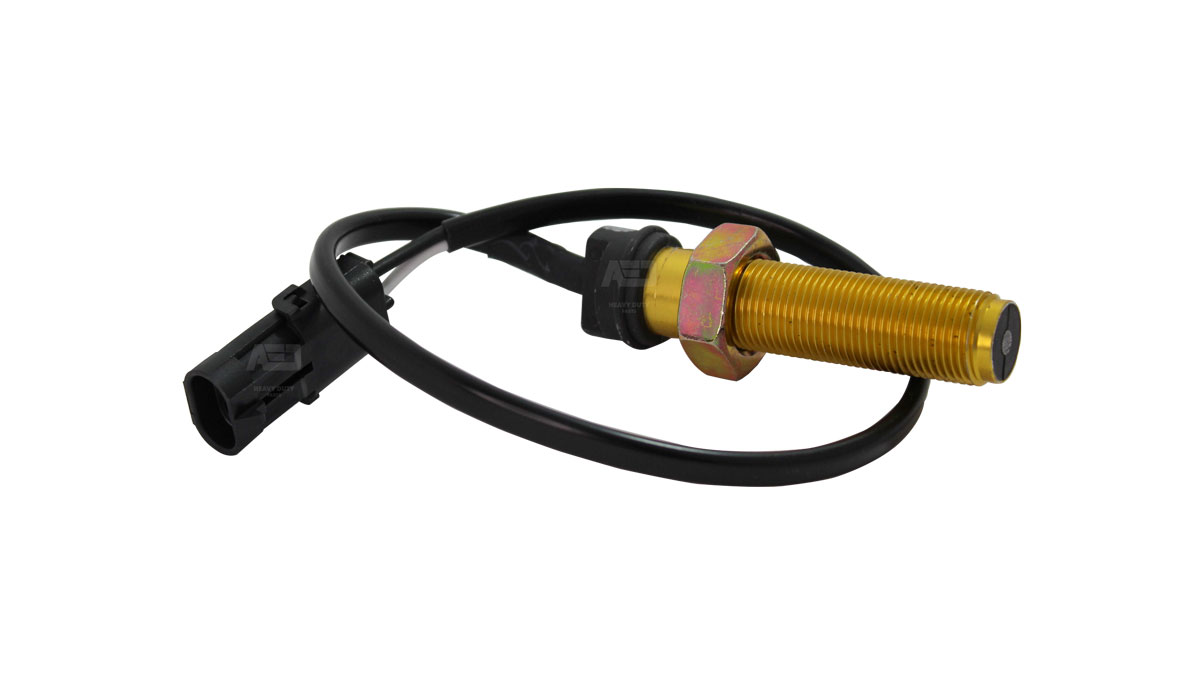
\includegraphics[width=0.5\linewidth, height=0.3\textheight]{img/tacometro}
	\caption[Tacometro]{}
	\label{fig:tacometro}
\end{figure}
	
	\textbf{Sensor de Efecto Hall:}
	
	Es un sensor de medición de velocidad el cual tiene el principio de “Si una pieza plana de material conductivo llamada chip Hall se sujeta a una diferencia de potencial en sus dos lados opuestos entonces el voltaje que se genera a través de las caras perpendiculares es cero”.\autoref{fig:hall}\\\\\\\\\\
	
	
\begin{figure}[h]
	\centering
	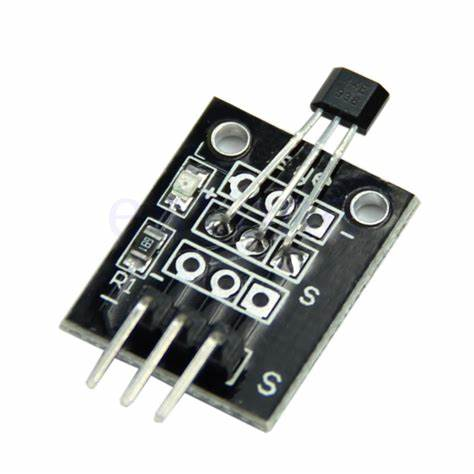
\includegraphics[width=0.2\linewidth, height=0.2\textheight]{img/HALL}
	\caption{}
	\label{fig:hall}
\end{figure}
	
	
	
	
	\textbf{Galgas extensométricas:}
	
	El principio de este sensor es que el alargamiento de un conductor aumenta su resistencia eléctrica. Este incremento de resistencia se debe a incremento de la longitud del conductor y decremento en el área del conductor.\autoref{fig:galga-extensiometrica-300x202}
	
\begin{figure}[h]
	\centering
	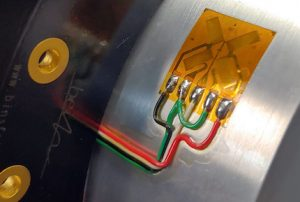
\includegraphics[width=0.3\linewidth, height=0.2\textheight]{img/galga-extensiometrica-300x202}
	\caption{}
	\label{fig:galga-extensiometrica-300x202}
\end{figure}

	\textbf{Interruptores piezoeléctricos:}

Son sensores que utilizan un material piezoeléctrico el cual señala que cuando cristales eléctricos asimétricos se deforman mediante una fuerza, se desarrolla un potencial eléctrico dentro de la red cristalina deformada. Son capaces de medir fuerzas, presiones, vibraciones y aceleraciones.\\\\\\\\\\\\

	
\begin{figure}[h]
	\centering
	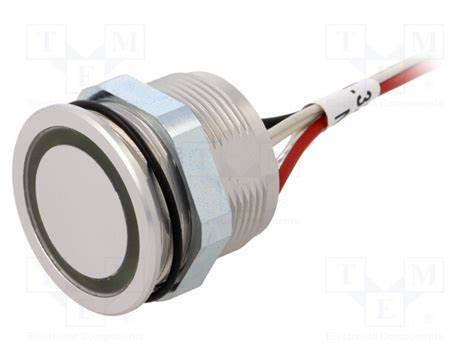
\includegraphics[width=0.3\linewidth, height=0.2\textheight]{img/S}
	\caption[f]{}
	\label{fig:s}
\end{figure}
